\documentclass[12pt,letterpaper,answers]{exam}
\usepackage[usenames,dvipsnames,svgnames,table]{xcolor}
\usepackage[margin=0.9in]{geometry}
\usepackage{tikz}
\renewcommand{\familydefault}{\sfdefault}
\usepackage{multicol}
\pagestyle{head}
\header{AM 111}{}{Skill Checks (Examples)}
\runningheadrule
\headrule
\usepackage{graphicx} % more modern
\usepackage{amsmath} 
\usepackage{amssymb} 
\usepackage{hyperref}
\usepackage{tcolorbox}

\begin{document}
 \pdfpageheight 11in 
  \pdfpagewidth 8.5in


\begin{enumerate}
\setcounter{enumi}{1}
\item (for Class 02)

Let $f(x) = 
\cos x$.  Find the condition number as a function of $x$.  Use relative error to construct your expression.

\begin{solution}
Using Taylor expansion to first order about $x$, $f(x+\Delta x)\approx f(x) + \Delta x \left.\dfrac{df}{dx}\right\vert_x$.

Working with a general $f(x)$:
$\text{cond }\# = \left\vert\dfrac{\hat{y}-y}{y} \right\vert / \left\vert\dfrac{\hat{x}-x}{x} \right\vert \approx \left\vert \dfrac{\Delta xf'(x)}{f(x)} \right\vert / \dfrac{\Delta x}{x} = \left\vert x\dfrac{f'(x)}{f(x)}\right\vert$

For $f(x) = \cos x$, we have

$\text{cond }\# \approx \left\vert x \dfrac{-\sin x}{\cos x} \right\vert  = \vert x\tan x\vert$

\end{solution}

\item (for Class 03)

Convert $12.35$ to binary.

\begin{solution}
    Convert the integer part and the decimal part separately.
    \begin{multicols}{2}
    
    $12 = 6*2 + 0$
    
    $6 = 3*2 + 0$
    
    $3 = 1*2 + 1$

    $1 = 0*2 + 1$
    
    So $(12)_{10} = (1100)_2 $
    
    \columnbreak
    
    $0.35 * 2 = 0.7 = 0.7 + 0$
    
    $0.7*2 = 1.4 = 0.4 + 1$
    
    $0.4*2 = 0.8 = 0.8 + 0$
    
    $0.8*2 = 1.6 = 0.6 + 1$
    
    $0.2*2 = 1.2 = 0.2 + 1$
    
    $0.2*2 = 0.4 = 0.4 + 0$
    
    $0.4*2 = 0.8 = 0.8 + 0$
    
    So $(0.35)_{10} = (0.01\overline{0110})_2$
    
    \end{multicols}
    
    Combining, $(12.35)_{10} = (1100.01\overline{0110})_2$
\end{solution}

\item (for Class 04)

Using $\left\{(x_i,y_i)\right\}_{i=1}^2 = \left\{(1,7), (2,4)\right\}$ as your data, and $f(x) = x^2$ as your model, 
\begin{parts}
\item construct the error vector $\vc{e}$, and
\item find the $1$-norm of $\vc{e}$
\end{parts}

\emph{You may be asked for the $1$-norm, $2$-norm, or $\infty$-norm of $\vc{e}$.}

\begin{solution}

$f(x_1) = 1^2 = 1$, $f(x_2) = 2^2 = 4$.  $\vc{e} = (7-1, 4-4) = (6,0)$.

The $1$-norm is $\vert 6\vert + \vert 0 \vert = 6.$

\end{solution}

\item (for Class 05) 

\begin{questions}
\item Given $A\vc{w} = \vc{y}$, with the system overdetermined, construct the normal equations for this system.

Let $A = \left[\begin{array}{r r}
1 & 3 \\
-2 & 1 \\
0 & 4
\end{array}\right]$ and $\vc{y} =  \left[\begin{array}{r}
4 \\ 2 \\ 5 \end{array}\right]$.  

\emph{You do not need to complete the matrix multiplications.}
\item The skill from the Class 01 handout (Skill Check C02).
\end{questions}


\begin{solution}
\begin{questions}
\item The normal equations are $A^TA\vc{w} = A^T\vc{y}$.  The solution, $\vc{w} = \vc{w}^*$, will be the closest solution to the original system under a least-squares error measurement.

The equations are

\[\left[\begin{array}{c c c}
1 & -2 & 0 \\
3 & 1 & 4
\end{array}\right]\left[\begin{array}{r r}
1 & 3 \\
-2 & 1 \\
0 & 4
\end{array}\right] \vc{w}^* = \left[\begin{array}{c c c}
1 & -2 & 0 \\
3 & 1 & 4
\end{array}\right] \left[\begin{array}{ r}
4 \\ 2 \\ 5\end{array}\right]\]

\item See the Class 01 handout for the example.
\end{questions}
\end{solution}

\item (for Class 06)

Write the quadratic form $Q(x_1,x_2,x_3) = x_1^2 + 4x_1x_3 - x_2x_3 + 7x_3^2$ as a matrix equation of the form $\vc{x}^TA\vc{x}$ where $A$ is a $3\times 3$ symmetric matrix.

\begin{solution}
The coefficients of $x_j^2$ go on the diagonal (so $1$, $0$, $7$ will be the diagonal).

To fill in $a_{12} = a_{21}$ use the $x_1x_2$ term (coefficient is zero).

To fill in $a_{13} = a_{31}$ use the $x_1x_3$ term (coefficient is $4$ so the matrix entries are each $2$).

To fill in $a_{23} = a_{32}$ use the $x_2x_3$ term (coefficient is $-1$ so the matrix entries are each $-1/2$).


$Q(\vc{x}) = \vc{x}^T\left[\begin{array}{r r r} 
1 & 0 & 2 \\
0 & 0 & -1/2 \\
2 & -1/2 & 7
\end{array}\right] \vc{x}$

We can multiply this out to check:

\begin{align*}
    Q(\vc{x}) &= \vc{x}^T\left[\begin{array}{c}
x_1 + 2x_3 \\
-x_3/2 \\
2x_1 - x_2/2 + 7x_3
\end{array}
\right] \\
&= x_1^2 + 2x_3x_1 - x_3x_2/2 + 2x_1x_3-x_2x_3/2 + 7x_3^2 \\
&= x_1^2 + 4x_1x_3 - x_2x_3 + 7x_3^2
\end{align*}
\end{solution}

\item (for Class 07)

Let $f(x) = x^2 -x -1$ and $x_0 = 0$.  Apply one step of Newton's method.

\begin{solution}
$x_1 = x_0 - f(x_0)/f'(x_0)$.  

$f'(x) = 2x - 1$.

$f(0) = -1$, $f'(0) = -1$.  $x_1 = 0 - -1/(-1) = -1$

$f(-1) = -1$, $f'(-1) = -3$.  $x_2 = -1 - -1/(-3) = -4/3$
\end{solution}

\item (for Class 08) For sufficiently large $k$, $\dfrac{\vert e_{k+1}\vert}{\vert e_k\vert^r} \approx C$


$C$ and $r$ are estimated from successive steps of a numerical algorithm below.

\begin{verbatim}
0.11369060817278044 3.329460092761372
0.1573815133502217 0.8941370047142863
1.3248374877542113 2.125788830275385
0.11466352084798608 1.4051502969581708
1.010392350228528 1.7188363535167348
0.18863719882541435 1.5779653647657021
\end{verbatim}

Assuming a simple root, is this sequence generated by the bisection method, Newton's method, or the secant method?

\emph{These sequences were generated via the Python code that we used in class during Class07}

\begin{solution}
In the later steps, $r\approx 1.5$, i.e. it is superlinear but not approaching quadratic.  This is the secant method.
\end{solution}

\item (for Class 09)
Consider the data points $(1,7)$, $(3, 5)$, $(4, 9)$.  Construct $L_{3,1}$, the Lagrange basis function of degree $2$ that is $1$ at $x_1 = 1$ and is $0$ at the other input values.

\begin{solution}
For zeros at $3$ and $4$, we have $(x-3)(x-4)$.  For the function to be $1$ at $x = 1$, we have $L_{3,1} = \dfrac{(x-3)(x-4)}{(1-3)(1-4)}$

\end{solution}

\item (for Class 10)

Use Lagrange interpolation to construct an approximation to $f(x) = \sqrt{x}$ based on the following data points: $(0,0)$,$(4,2)$, $(9,3)$.

Identify the degree of your interpolating polynomial.

\begin{solution}
First construct the basis functions:

$l_1(x) = \dfrac{(x-4)(x-9)}{(0-4)(0-9)}$

$l_2(x) = \dfrac{(x-0)(x-9)}{(4-0)(4-9)}$

$l_3(x) = \dfrac{(x-0)(x-4)}{(9-0)(9-4)}$

Then construct the polynomial interpolant:
$P(x) = 0l_1(x) + 2l_2(x) + 3l_3(x)$

It turns out that if $y_i = 0$ then there is no need to construct $l_i$.

This polynomial is degree $2$.

\end{solution}

\item (for Class 11)

Decide whether the equations form a cubic spline.

\[S(x) = \left\{\begin{array}{l l}
x^3 + x - 1 & \text{on }[0,1] \\
-(x-1)^3 + 3(x-1)^2 + 3(x-1) + 1 & \text{on }[1,2] \\
\end{array}\right.\]

\begin{solution}

$S_1(1) = 1+1-1 = 1$

$S_2(1) = 0 + 0 + 0 + 1 = 1$

So $S(x)$ is continuous.

$S_1'(x) = 3x^2 + 1$ and $S_2'(x) = -3(x-1)^2 + 6(x-1) + 3$.

$S_1'(1) = 3 + 1 = 4$

$S_2'(1) = 0 + 0 + 3$

So $S'(x)$ is not continuous and $S(x)$ is not a cubic spline.
\end{solution}

\item (for Class 12)

Let $f(x) = x^3 - 3x$.  Write an expression for $f'(x)$ approximated using central differences at $x_0 = 2.0$ with $h = 0.01$.

\emph{You will be asked for one of forward differences, central differences, or backward differences.}
\begin{solution}
 The formula is $(f(x+h) - f(x-h))/(2h)$ so $\dfrac{2.01^3-3*2.01 - 2^3+3*2}{0.02}$.
\end{solution}

\item (for Class 13/14)

Using Taylor expansion, it is possible to show that \[f''(x) = \dfrac{f(x-h)-2f(x)+f(x+h)}{h^2} - \frac{1}{12}h^2 f''''(x) + \mathcal{O}(h^6).\]

Identify the order of the method if 
\[f''(x) \approx \dfrac{f(x-h)-2f(x)+f(x+h)}{h^2}\]
is used to approximate the second derivative.

\begin{solution}
The order of the method comes from the first error term, which is $\frac{1}{12}h^2f''''(x)$, so this is a second order method.
\end{solution}

\setcounter{enumi}{14}
\item (for Class 15)

Find the degree of precision of the following approximation for $\displaystyle\int_{-1}^1 f(x)dx$:
% $f(1)+f(-1)$, 
%$\dfrac{2}{3}[f(-1)+f(0)+f(1)]$, %$f\left(\dfrac{1}{\sqrt{3})\right) + f\left(\dfrac{1}{\sqrt{3})\right)$

$\displaystyle\int_{-1}^1 f(x)dx\approx 2f(0)$.

\emph{The following information may be helpful}
\[\int_{-1}^1 1\ dx = 2, \int_{-1}^1 x\ dx = 0, \int_{-1}^1 x^2\ dx = \frac{2}{3}, \int_{-1}^1 x^3\ dx =0, \int_{-1}^1 x^4\ dx = \frac{2}{5}\]

\begin{solution}
For $f(x) = 1$, $2f(0) = 2$ so this is exact for $f$ constant.

For $f(x) = x$, $2f(0) = 0$ so this is exact for $f$ linear.

For $f(x) = x^2$, $2f(0) = 0$, which does not match.

The degree of precision is $1$.
\end{solution}


\item (for Class 16)

The error from using the midpoint rule to approximate $\int_a^b f(x)dx$ with a single panel is given by $-\frac{1}{24}h^3f''(c_1)$, where $h$ is the panel size.  What is the error for the composite rule?

\begin{solution}
$-\frac{1}{24}(b-a)h^2f''(c)$.  

Explanation:
For $m$ panels evenly splitting $[a,b]$, this comes from $\sum\limits_{k=1}^m -\frac{1}{24}h^3f''(c_k) = -\frac{1}{24}mh^3f''(c) = -\frac{1}{24}(b-a)h^2f''(c)$ (from the generalized intermediate value theorem and noting $mh = (b-a)$).

In general for error $\alpha h^nf''(c_1)$ on a single panel, the error will be $\alpha (b-a)h^{n-1}f''(c)$ for the composite rule.
\end{solution}

\item (for Class 17)

A quadrature rule can be written in the form $\sum\limits_{k=1}^n a_k f(x_k)$. For the composite midpoint rule on two panels, given by $(b-a)\frac{1}{2}\left(f(a + \frac{b-a}{4})+ f(a + 3\frac{b-a}{4})\right)$, identify $n$ and $a_k, x_k$ for $k=1,...,n$.

%Trapezoid rule: $(b-a)\frac{1}{2}(f(a)+f(b)$
%Simpson's rule
% Gauss quadrature 

\begin{solution}
There are two points in the calculation so $n = 2$.
$a_k = \frac{1}{2}(b-a)$ for both points.  $x_1 = a+(b-a)/4$. $x_2 = a+3(b-a)/4$.
\end{solution}


\item (for Class 18)

A particular quadrature rule for $\displaystyle\int_0^4f(x)dx$ is given by fitting a parabola to $(0,f(0)), (1,f(1)), (2,f(2))$, fitting a second parabola to $(2,f(2)), (3,f(3)), (4,f(4))$, and integrating the fitted curves.

This is a composite (or adaptive) method:
\begin{oneparchoices}
\choice yes \choice no
\end{oneparchoices}

This is a Newton-Cotes method:
\begin{oneparchoices}
\choice yes \choice no
\end{oneparchoices}

How do you know?

\begin{solution}
For a composite or adaptive method we would see multiple panels.  A parabola is being fit separately to two sub-regions, so this is a composite method.  

For a Newton-Cotes method, the quadrature points are evenly spaced on the interval, as they are here.

Yes and yes.
\end{solution}


\item (for Class 19)

Consider the initial value problem $\left\{\begin{array}{l}
y' = -2y \\
y(-2) = 5
\end{array}
\right.$

Set $h = 0.1$.  Provide an expression for $y(-2+0.1)$, as approximated using improved Euler/trapezoid.

\begin{solution}
In Euler's method, $w_0 = 5$, $w_1 = 5 + 0.1f(-2,5)$.

$f(-2,5) = -10$ so $w_1 = 5+0.1(-10) = 4$.  

$f(-1.9,4) = -8$

For improved Euler, use $w_0 + 0.1 \frac{1}{2}(f(-2,5) +f(-1.9,4)) = 5+0.1(-10-8)/2$.

\emph{Improved Euler gives $4.1$ while Euler gives $4$.}
\end{solution}


\item (for Class 20)

The midpoint method is given by $y_{k+1} = y_k + h\psi(t_k,y_k,h)$ where $\psi(t_k,y_k,h) = f(t_k+h/2,y_k+hf(t_k,y_k)/2)$.

Use Taylor expansion to first order to write $f(t_k+h/2,y_k+hf(t_k,y_k)/2)$ in terms of $f(t_k, y_k)$,$\dfrac{\partial f}{\partial t}(t_k,y_k)$, $\dfrac{\partial f}{\partial y}(t_k,y_k)$, and $\mathcal{O}(h^2)$.

\begin{solution}
Taylor expanding about $f(t_k, y_k)$, the displacement in time is $\Delta t = h/2$ and the displacement in $y$ is $\Delta y = hf(t_k,y_k)$.

In general, $f(t+\Delta t, y+\Delta y) = f(t,y) + \Delta t \dfrac{\partial f}{\partial t}(t,y) +  \Delta y \dfrac{\partial f}{\partial y}(t,y) + \text{higher order terms}$


Applying this:

$f(t_k+h/2,y_k+hf(t_k,y_k)/2) = f(t_k,y_k) + \dfrac{h}{2} \dfrac{\partial f}{\partial t}(t_k,f_k) + \dfrac{h}{2}f(t_k,y_k) \dfrac{\partial f}{\partial x}(t_k,f_k) + \mathcal{O}(h^2)$

\end{solution}


\item (for Class 21)

There are $s = 132300$ data points in a data set with $3$ seconds of data.  Find the frequency associated with the $33$rd Fourier mode ($c_{33}$) in units of $1/$seconds (Hertz).

\begin{solution}
This is the frequency associated with $33$ cycles (cosine or sine waves) in time $3$ seconds, which is $11$ cycles per second, or $11$ Hertz $(33/3)$.
\end{solution}


\item (for Class 22)

Match the signal to its DFT amplitude.  Provide reasoning.

Signal:

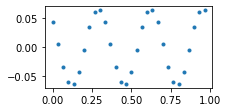
\includegraphics[width=0.3\linewidth]{img/C21skill.png}

Frequency options:

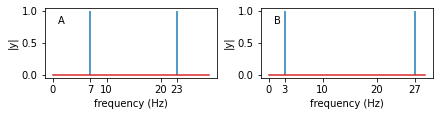
\includegraphics[width=0.7\linewidth]{img/C21skill2.png}

\begin{solution}
The options for frequency are at 7 Hz or a 3 Hz.  Three sinusoid periods is about right for this signal (definitely not 7 periods).  So option B.
\end{solution}


\item (for Class 23)

For the neural network below, how many inputs does it have?  How many units in the first hidden layer?  What is the depth of the network?

\newcommand{\inputnum}{2} 
% Hidden layer neurons'number
\newcommand{\hiddennum}{3} 
% Hidden layer neurons'number
\newcommand{\hiddennumk}{4}  
% Output layer neurons'number
\newcommand{\outputnum}{1} 
\begin{tikzpicture}
% Input Layer
\foreach \i in {1,...,\inputnum}
{
    \node[circle, 
        minimum size = 6mm,
        fill=orange!30] (Input-\i) at (0,-\i) {};
}
% Hidden Layer
\foreach \i in {1,...,\hiddennum}
{
    \node[circle, 
        minimum size = 6mm,
        fill=teal!50,
        yshift=(\hiddennum-\inputnum)*5 mm
    ] (Hidden-\i) at (2.5,-\i) {};
}
\foreach \i in {1,...,\hiddennumk}
{
    \node[circle, 
        minimum size = 6mm,
        fill=teal!50,
        yshift=(\hiddennumk-\inputnum)*5 mm
    ] (Hiddenk-\i) at (5,-\i) {};
}
% Output Layer
\foreach \i in {1,...,\outputnum}
{
    \node[circle, 
        minimum size = 6mm,
        fill=purple!50,
        yshift=(\outputnum-\inputnum)*5 mm
    ] (Output-\i) at (7.5,-\i) {};
}
% Connect neurons In-Hidden
\foreach \i in {1,...,\inputnum}
{
    \foreach \j in {1,...,\hiddennum}
    {
        \draw[->, shorten >=1pt] (Input-\i) -- (Hidden-\j);   
    }
}
% Connect neurons Hidden-Out
\foreach \i in {1,...,\hiddennum}
{
    \foreach \j in {1,...,\hiddennumk}
    {
        \draw[->, shorten >=1pt] (Hidden-\i) -- (Hiddenk-\j);
    }
}
\foreach \i in {1,...,\hiddennumk}
{
    \foreach \j in {1,...,\outputnum}
    {
        \draw[->, shorten >=1pt] (Hiddenk-\i) -- (Output-\j);
    }
}
% Inputs
\foreach \i in {1,...,\inputnum}
{     
    \draw (Input-\i) node {$x_{\i}$};
    % \draw[<-, shorten <=1pt] (Input-\i) -- ++(-0.5,0)
    %     node[left]{$x_{\i}$};
}
% Outputs
\foreach \i in {1,...,\outputnum}
{            
\draw (Output-\i) node {$y_{\i}$};
    % \draw[->, shorten <=1pt] (Output-\i) -- ++(0.5,0)
    %     node[right]{$y_{\i}$};
}
\end{tikzpicture}

\begin{solution}
Two inputs ($x_1$ and $x_2$), three units in the first hidden layer, and a depth of three (the input layer isn't counted in the depth).
\end{solution}


\end{enumerate}
\end{document}